\section{Introduction} \label{sec:intro}

Recently, Virtual Reality (VR) becomes increasingly more popular. It enables a wide array of novel applications in many domains, such as computer games, occupational training, healthcare, manufacturing, etc. The market research also reports that foresee explosive growth of the VR market in the upcoming years~\cite{XR_market}.

One way to classify the VR applications is through the different {\em interaction techniques}. Because of the high popularity of 360{\degree} video streaming services, most users are familiar with the {\em 3DoF} (Degree-of-Freedom) interactions, in which a user's viewport is determined by his/her head/HMD {\em orientation}. 3DoF interactions, however, assume that the user does not change his/her {\em positions}. That is, when a user of a 3DoF VR application stands up and walks around, his/her HMD viewport would not reflect the changes of positions. Therefore, the user will {\em not} feel he/she is moving in the virtual world, leading to inferior {\em immersive} user experience. {\em 6DoF} interactions address the above limitations by rendering  the position-dependent viewports to the user's HMD when he/she walks around. Fig.~\ref{fig:vr_phase} illustrates the difference between 3DoF and 6DoF interactions.

% \begin{figure}[tbh]
%     \centering
%     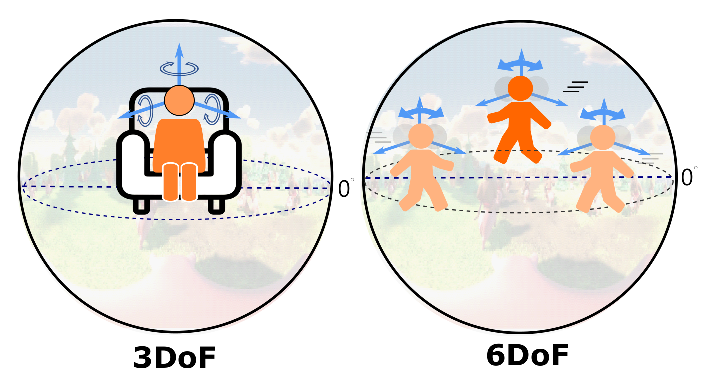
\includegraphics[width=0.46\textwidth]{figs/vr_phase}
%     \caption{Difference between 3DoF and 6DoF interactions.}
%     \label{fig:vr_phase}
% \end{figure}

Supporting 6DoF XR using 360{\degree} videos is not an easy task, because for every single position, a new 360{\degree} video needs to be captured. Even if we deploy dense 360{\degree} cameras, user may still miss smooth transitions at the positions between any two adjacent cameras. Hence, more descriptive 3D representations are required for enabling the truly immersive experience of 6DoF VR applications. Recently, MPEG-I (Moving Picture Expert Group--Immersive Group) has been actively developing MPEG Immersive Video (MIV) standard~\cite{BDDF+21, MPEG_MIV_web}. It use multi-view RGB-D video as the data representation, and including the entire pipeline for encoding, decoding, and rendering. The Test Model for Immersive Video (TMIV)~\cite{tmiv_doc,tmiv_gitlab}, which is the reference software of MIV standard, has been released to show a reference implementation of MIV.

In this paper, we conduct a series of experiments to evaluate the performance of the latest version of TMIV. We capture several video sequences with various camera placement in different scenes, and running TMIV with different set of parameters. 
This paper makes the following contributions:
\begin{itemize}
    \item We implement a video sequence capturing system. The system can capture view from any position and orientation, and automatically generate the config file of camera parameter for TMIV. It benefits the scenario which needs a huge amount of data, e.g., training a machine learning model for immersive video application. 
    \item We consider several camera placements in our experiments. The results of our experiments can be utilized or extended to find camera placement with higher performance.
    \item We consider several parameters in TMIV codec, e.g, number of groups, depth estimation, and synthesizer in TMIV. The results of our experiment show the performance of TMIV in various scenarios. The results may inspire the future application of TMIV.
\end{itemize}

% The rest of this paper is organized as follows. We survey the related work in Sec.~\ref{sec:related}, and giving an introduction for MIV standard in Sec.~\ref{sec:TMIV}. Sec.~\ref{sec:implementation} introduce our implementation for experiments. The setup and results of our experiments are shown in Sec.~\ref{sec:experiment}. Finally, we conclude this paper and list some future work in Sec.~\ref{sec:conclusion}
